This chapter focuses on the modelling of the atomic elements of the robot. We begin by explaining how to create the model of an object inside V-Rep. We then show how to use to model simple elements such as frames or electronics who are not active during the simulation i.e. they do not perform any function. Those can be represented strictly mechanically. We then show how to model active pieces such as the cameras of the servos before finally presenting a complete model of a robot.

\section{Problem statement}
Our robot will be made from a number of elements that all need to be represented in the simulation:\begin{itemize}
\item \textbf{Miscellaneous mechanics and electronics:} A type of element that must be included in the model are the frames, \Cref{fig:fr07-h101} shows the FR07-H101 frame. On the actual robot, they will link the servos together. Other mechanical elements are the hands, the feet and the plate that will act as the trunk of the robot. 

In addition to all the aforementioned elements we plan to equip the legs of the robot with springs. Their purpose will be to make the robot walk more efficiently by storing energy in these springs when the foot hits the ground and releasing it when the leg takes another swing.

The robot will also have an array of electronic elements. An Intel Atom processor (\Cref{fig:smarc}) to perform the high-level control (giving target angles to the servomotors, computing trajectories, processing the inputs from the cameras, etc),  batteries to stock the energy necessary to power them and the electronics to convey that energy through the robot.

\item \textbf{Cameras:} The robot will be equipped with two cameras of the type shown in \Cref{fig:li_cam}. Situated at the top of the robot, it will use them to locate itself and points of interest in the play arena\footnote{This is the subject of an on-going master thesis at Montefiore.}. As we may test some machine vision algorithms during our (future) simulations we need to have the ability of retrieving the image or a video stream a camera captures.

\item \textbf{Servomotors:} We will be using the MX-28R servo, shown in \Cref{fig:mx28}, as the driving element of the joints of the robot. We need to represent it as a rigid body as well as its function as a mechanical device that can generate torque on its axle to keep a targeted angle (hence the name \emph{servo}, from the Latin word for \emph{slave}).
\end{itemize}

\begin{figure}[htp]
\center
    \begin{subfigure}[b]{0.4\textwidth}
    \center
    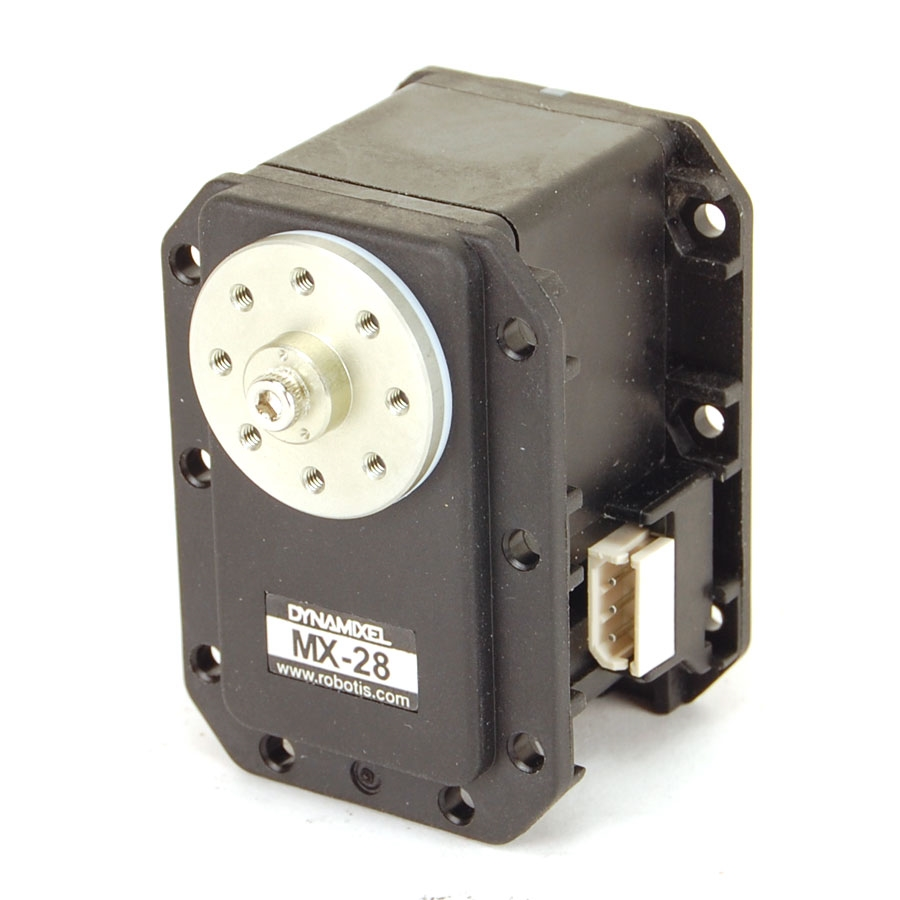
\includegraphics[width = \textwidth]{figures/mx28}
    \caption{MX-28R servo. \label{fig:mx28}}
    \end{subfigure}
    \hfill
    \begin{subfigure}[b]{0.4\textwidth}
    \center
    \includegraphics[width = \textwidth]{figures/fr07-h101}
    \caption{FR07-H101 hinge type frame. \label{fig:fr07-h101}}
    \end{subfigure}

    \begin{subfigure}[b]{0.4\textwidth}
    \center
    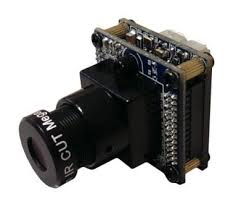
\includegraphics[width = \textwidth]{figures/li_cam}
    \caption{LI-USB30-M021C camera. \label{fig:li_cam}}
    \end{subfigure}
    \hfill
    \begin{subfigure}[b]{0.4\textwidth}
    \center
    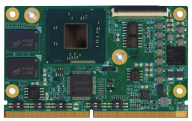
\includegraphics[width = \textwidth]{figures/smarc}
    \caption{SMARC Short Size Module. \label{fig:smarc}}
    \end{subfigure}
    \caption[Atomic elements of our robot]{Atomic elements of our robot. The MX-28R and the camera are more complex to model as they each perform a function in the simulation. On the other hand, the frame and the motherboard are only dead weight.}
    \label{fig:modelling_problem}
\end{figure}

\section{Modelling in V-Rep \label{sec:modelling}}
This section is a short introduction to the creation of a dynamic model of an object in V-Rep. We present how to set its mass, inertia and friction and how to make it collide with other models and respond to forces. Later, we present how to create constraints between models and explain why it is useful.

\subsection{Creating the model of an object}
The creation of a rigid body inside V-Rep begins with the creation of a mesh\footnote{an ensemble of vertices and faces that represent an object} in a modelling tool which in our case is Blender. It is preferred to have a convex mesh, i.e. one that whose all interior meshes are less or equal to $180\degree$, as they are easier for the simulator to handle. When it is absolutely necessary to keep the mesh concave, a solution is to separate it into several convex meshes that will be grouped together in V-Rep. Once saved in a file format recognized by V-Rep the mesh can be imported into the latter. 

\begin{figure}[htp]
\center
    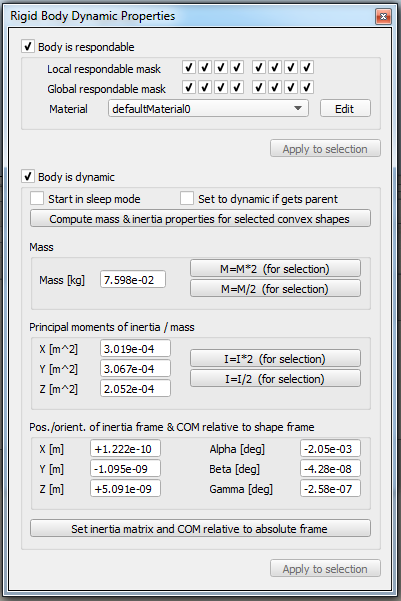
\includegraphics[width = 0.6\textwidth]{figures/v-rep_modelling}
    \caption[Rigid body dynamic properties]{Configuration window of the dynamic properties of the selected rigid body. We can make it \emph{respondable}, i.e. it should collide with other objects. We can also make it \emph{dynamic} in which case it will be dynamically active in the simulation and react to forces. When dynamically active, the movement of this body will be influenced by its \emph{mass} and its \emph{inertia}. It is also possible to set what is called \emph{Material} by V-Rep which is a set of parameters such as the friction of the material or its restitution parameter.}
    \label{fig:vrep_modelling}
\end{figure}

In V-rep, we open the properties of the mesh (the window in \Cref{fig:vrep_modelling}) and mark it as dynamic, respondable (if necessary) and set the mass and the inertia. It is possible to have V-Rep compute it automatically from the geometry and the density but it can also be set manually.

\subsection{Creating constraints between models \label{sec:joints}}
In V-Rep the constraints exist under the form of \emph{joints}. There exist three types of joints:\begin{enumerate}
\item \textbf{Revolute joints:} they have 1 degree of freedom (DOF) and enforce rotational movements between objects. The range of the rotation around the axis of the joint can be restricted. By default, it is passive but it can be set to \emph{torque/force mode} where it will try to hold a target angle, very much like a servomotor would.
\item \textbf{Prismatic joints:} they have 1 DOF and enforce rotational translational movements between objects. As in the case of the revolute type of joint, the range can also be restricted. There also exist a torque/force mode setting but in the case of a prismatic joint its purpose is to represent a spring-damper. The stiffness and damping can be specified in the properties of the joint.
\item \textbf{Spherical joints:} they have 3 DOF and enforce rotational translational movements between objects. Spherical joints do not have a torque/force mode and can only be passive. 
\end{enumerate}
A very important characteristic of joints is that they must link two dynamic objects together in order to work properly during the simulation. Two joints cannot be directly connected one to another.

\section{Modelling the miscellaneous mechanical elements and electronics}
The modelling of most of the mechanical elements and electronics is rather straightforward but there are some where the process is more troublesome. This is the case of the feet, frames and springs, and those will be detailed hereunder after a short explanation of the modelling process of the simpler pieces.

\subsection{Modelling the electronics, batteries, hands and the central plate}
The modelling of electronics, batteries, hand and central plate consists in applying the procedure explained in \Cref{sec:modelling}. These elements are already pretty simple in reality as they all have cuboid shapes. All their dimensions and weights are in \Cref{table:weights} along with a suggested material in the case of pieces that will have to be custom made.

\begin{table}[htp]
\centering
\begin{tabularx}{\textwidth}{@{} l l X X p{4.1cm} @{}}
\toprule
\textbf{Module} & \textbf{Weight [$g$]} & \textbf{Material} &  \textbf{Density [$kg/m^3$]}& \textbf{Dimensions $x[mm] \cdot y[mm] \cdot z[mm]$}\\ 
\midrule
Odroid C-2 & 40 & [-] & 840 & $85.0 \cdot 56.0 \cdot 10.0$\\
Li-Po battery & 188 & Li-Po & 2304 & $103.0 \cdot 33.0 \cdot 24.0$\\
Hand & 30 & Aluminium & 3000 & $70.0 \cdot 31.0 \cdot 31.0$\\
Feet & 52 & Polymer & 1000 & $70.0 \cdot 125.0 \cdot 6.0$\\
Central plate & 209 & Aluminium & 4000 & $140.0 \cdot 30.0 \cdot 124.5$\\
\bottomrule
\end{tabularx}
\caption[Weights and dimensions of the pieces of the robot]{Weights and dimensions of the pieces of the robot. The density is useful for the automatic computation of the weight and inertia of the pieces in V-REP. The differences in density between different pieces made of the same material represent the differences in geometry, i.e. pieces with holes in them that are not modelled but taken into account by making the piece lighter.}
\label{table:weights}
\end{table}

\subsection{Modelling the feet}
In essence, the feet of our robot will be plates that will be fixed to the last servos of the legs. Contrary to other elements, feet \emph{must} be respondable as they come into contact with the floor. It follows that the friction parameter will be important too and it will have to be chosen in accordance to the friction parameter of the material they will be made of.

It should be noted that for the needs of the simulation, their z dimension has been exaggerated up to $6mm$ because of collision problems (sometimes, the contact point was on the upper side of the feet while it should have been on the down side) that disturbed the course of the simulation. Therefore, the z dimension reported in \Cref{table:weights} is the double of the actual one and the density has been halved to keep the same mass.

\subsection{Frames}
By \emph{frame} we mean the mechanical element that is used to connect the axle of a servo to another object which may be another servomotor. The frame in \Cref{fig:fr07-h101} is the standard one that will be part of the robot.

Frames are not directly present in the simulation. By that we mean that the link between the servomotors are made through joints without the intermediary of a frame. This reduces the accuracy of the model a bit but not by much. In exchange, we gain in speed and stability by reducing the number of constraints and not having a convex shape in the model of the robot.

\subsection{Springs}
As mentioned in \Cref{sec:joints} a spring can be represented by a prismatic joint. We link two objects together and set the joint to force/torque mode and we specify the stiffness and damping.

This is not enough if we want to model a spring that is between two elements that should be able to move not only in direction of the axis of the joint. For that purpose we add two spherical joints at the extremities of the prismatic joint. As it is impossible to link two joints together, we must add some intermediary objects between them. They are the objects called \emph{spring\_anchors} in \Cref{fig:spring2}.

Another problem we have to solve is that we have to create a loop inside the hierarchy of the model in order to connect a spring between two elements in a leg. V-Rep provides the ability of closing loops like this through \emph{dummy} objects (visible in \Cref{fig:spring2}). A pair of objects like these can be ordered to keep the same position. 

Now, in the case of the spring in \Cref{fig:springs}, we can attach it to a leg by moving it to the desired position and by making the \emph{Spherical\_joint5} a child of the element that is higher in the leg and \emph{Dummy4} a child of the element that is lower in the leg.

\begin{figure}[htp]
\center
    \begin{subfigure}[b]{0.45\textwidth}
    \center
    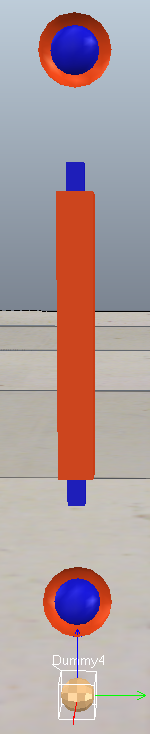
\includegraphics[height = 0.5\textwidth]{figures/springs}
    \caption{Visual representation of a spring in V-Rep. \label{fig:spring1}}
    \end{subfigure}
    \hfill
    \begin{subfigure}[b]{0.45\textwidth}
    \center
    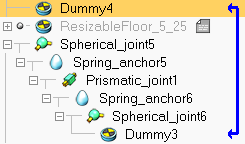
\includegraphics[height = 0.5\textwidth]{figures/springs_hierarchy}
    \caption{Hierarchy of the elements constituing the spring on \Cref{fig:spring1}. \label{fig:spring2}}
    \end{subfigure}
\caption[Modelling a spring]{Representation of a spring that can connect two elements of the same leg.}
\label{fig:springs}
\end{figure}

\section{Modelling the cameras}
As mentioned earlier, our robot will have two cameras at the top of its body. We are currently experimenting with cameras of the type illustrated in \Cref{fig:li_cam}. As far as the shape goes, the camera are modelled as cubes which dimensions and weights are in \Cref{table:cam_specs}.

\begin{table}[htp]
\center
\begin{tabularx}{\textwidth}{@{}X X X @{}}
\toprule
 & \textbf{Data} & \textbf{Unit}\\ 
\midrule
Weight & 22 & $g$\\
Dimensions & 26.0 x 26.0 x 14.7 & $mm^3$\\
Density & 2213 & $kg/m^3$\\
\bottomrule
\end{tabularx}
\caption[Characteristics of the LI-USB30-M021C camera]{Characteristics of the LI-USB30-M021C camera}
\label{table:cam_specs}
\end{table}

The active part of the camera, capture of videos and images, is simulated by a \emph{vision sensor}. As the name implies, this sensor captures what it sees. It has an array of properties, as shown in \Cref{fig:camera_model}, which influences what it can \emph{see exactly}. Some of them are rather performance related but we have access to the most essential parameters a camera has: the focal length and its resolution.

The possibility of embedding image processing is very interesting as by default the vision sensor captures the exact image of the world it sees. Therefore, a script can modify that image to be closer to what the actual camera would capture. For example, if the camera captured blurry images, a blur filter could be embedded in the vision sensor.

\begin{figure}[htp]
\center
    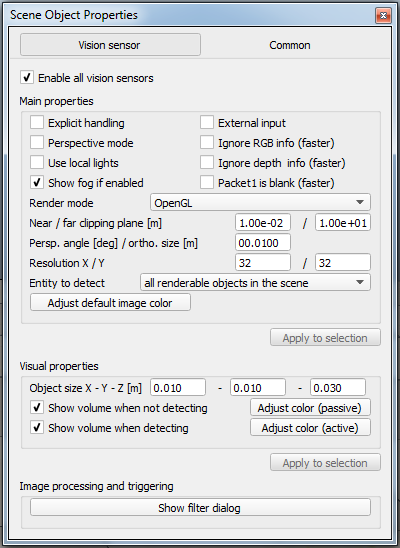
\includegraphics[width = 0.6\textwidth]{figures/v-rep_camera}
    \caption[Settings of vision sensor]{Properties of a vision sensor. We can set how far and how close it can see, which can be useful for performance. We can also set its resolution and the focal length (persp. angle [deg]/ortho. size[m] option). The \emph{show filter dialog} at the bottom gives the possibility to embed image processing scripts which could be useful in tuning the output of the camera.}
    \label{fig:camera_model}
\end{figure}

\clearpage
\section{Characterizing and modelling the MX-28R servomotor}
This section explains how the characteristics of the MX-28R servo are determined in order to make a physically accurate model of it. We will experimentally determine its torque and rotation speed.

\subsection{Determining the continuous torque}
The primary parameter we must know the value of to properly model the MX-28R is the torque it generates. The manual (\cite{mx_28_manual}) provides the value of the stall torque ($2.5Nm$ @$12V$) and a graph showing the efficiency of the servo at different torques and speeds but it does not provide a value of the actual continuous torque. We thus compute it from the maximal torque of the DC motor and the reduction ratio of the gears. 
\begin{align*}
ContinuousTorque &= TorqueMotor \times ReductionRatio\\
&= 3.67e^{-3} \times 193\\
&= 0.7083Nm
\end{align*}
The continuous torque is thus equal to $0.7Nm$.

\subsection{Determining the stall torque}
The stall torque is determined through a small experiment with a real MX-28R. The experimental setup is explained in \Cref{fig:exp_setup}. The experiment itself is presented in \Cref{fig:exp1}.

\begin{figure}[htp]
\centering
    \begin{subfigure}[b]{0.45\textwidth}
    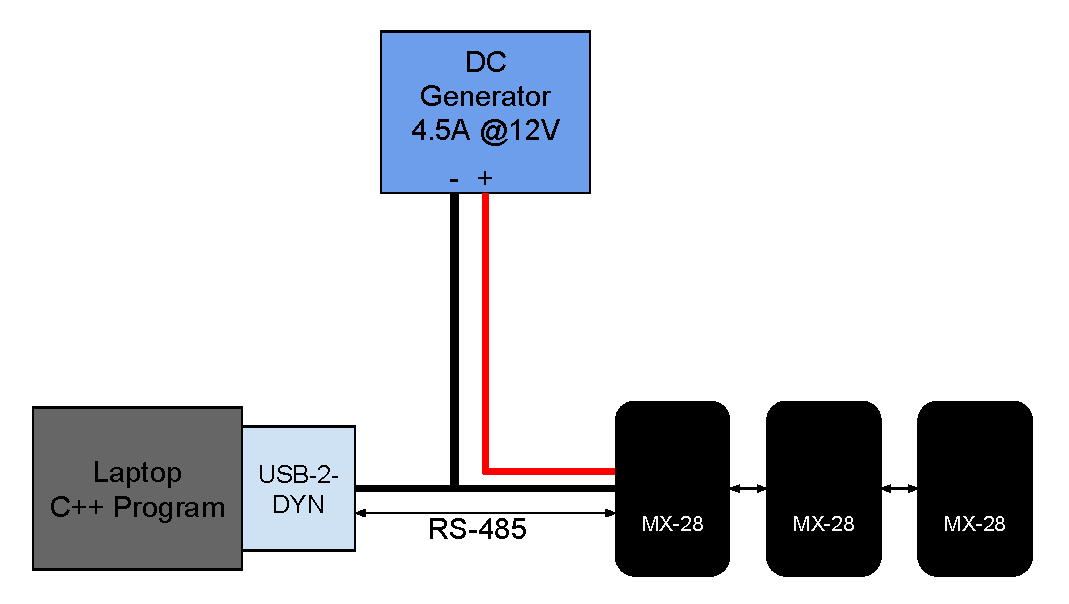
\includegraphics[width=\textwidth]{figures/exp_setup}
    \caption[Experimental setup]{The MX-28 servos are powered by a DC generator and controlled by a laptop equipped with a USB2DYNAMIXEL(USB-2-DYN) device.}
    \label{fig:dc_chain}
    \end{subfigure}
    \hfill
    \begin{subfigure}[b]{0.45\textwidth}
    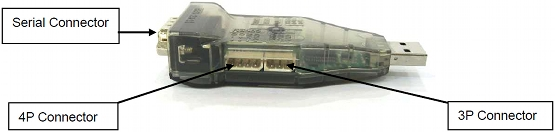
\includegraphics[width = \textwidth]{figures/u2d}
    \caption[USB2DYNAMIXEL]{A USB2DYNAMIXEL. It turns an USB port into a serial port (RS485, TTL or classic serial connector) that can be used to control Dynamixel manufactured servos. Source: \cite{usb2dyn_manual}}
    \label{fig:usb2dyn}
    \end{subfigure}
    \caption{Experimental setup \label{fig:exp_setup}}
\end{figure}

\begin{figure}[htp]
\centering
    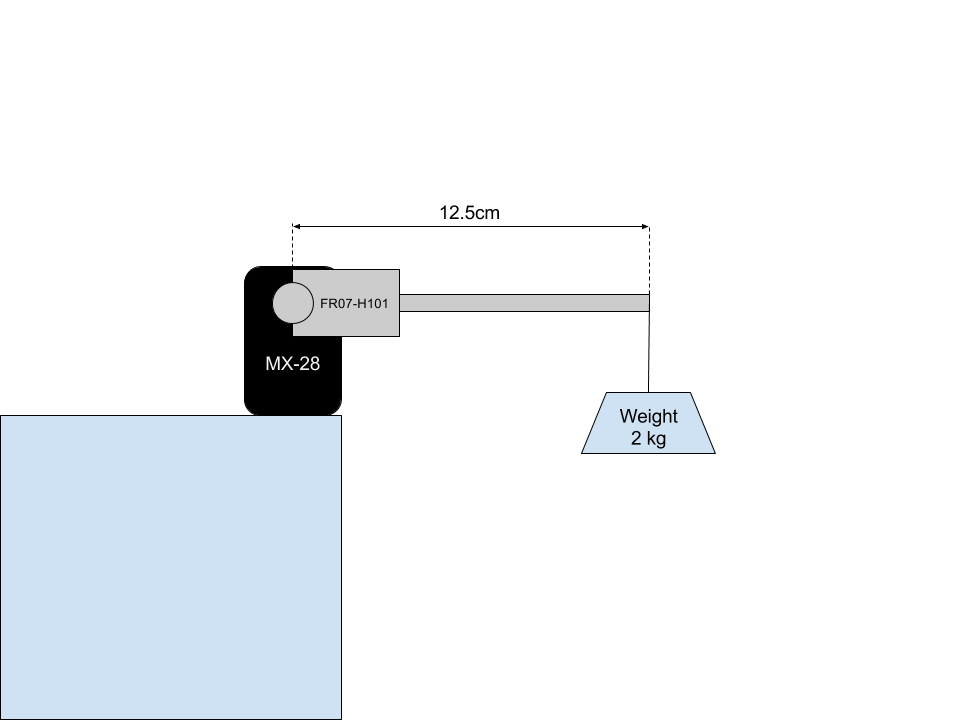
\includegraphics[width = 0.5\textwidth]{figures/exp1}
    \caption[Experimental setup for torque testing]{Experimental setup for torque testing. A weight $w$ is suspended at distance $d$ from the servo, resulting in an applied torque of $w \times g \times d$. $w$ is augmented until the servomotor is unable to lift the arm at which point we have determined the maximal torque it can generate.}
    \label{fig:exp1}
\end{figure}

\begin{figure}[htp]
\centering
    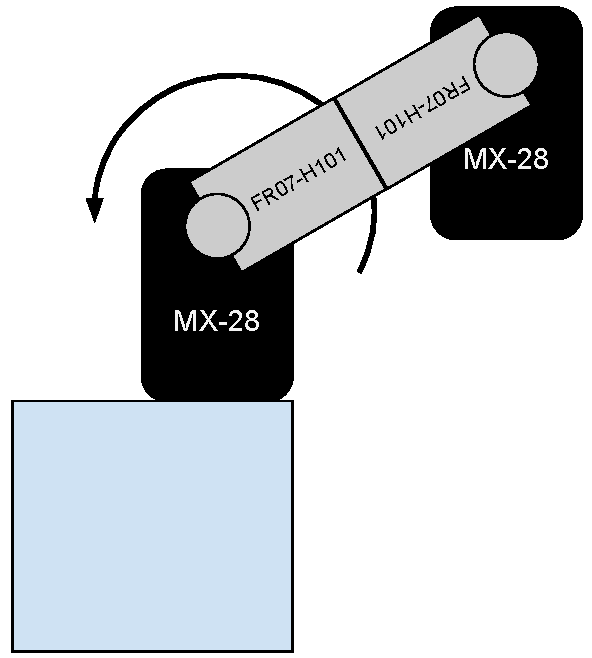
\includegraphics[width = 0.3\textwidth]{figures/exp2}
    \caption[Experimental setup dynamics testing]{Experimental setup for dynamics testing. One servo lifts the other. The goal is the measure the time it takes to swing the arm from $0\degree$ to $180\degree$.}
    \label{fig:exp2}
\end{figure}

In our case, $d$ was equal to $22.5cm$ and we could reach a weight $w$ of $740g$ at $14.8V$. This equals to a torque of $1.64Nm$. The complete results are in \Cref{table:mx28-specs}.

\subsection{Determining the rotation speed}
The goal of this experiment is to determine the unloaded rotation speed of the MX-28R. The setup is shown in \cref{fig:exp2}. The measuring is done by taking advantage of the rotary encoder inside the servomotor: we can measure the time it takes for the servo to go from $0\degree$ to $180\degree$ through a program.

The result is that executing this manoeuvre at $12V$ with no imposed speed limit takes $620msec$. This corresponds to a rotation speed of $48.33$ rotations per minute (Rpm).

\subsection{Results}
The results of all the previous experiments along with the characteristics of the MX-28R servomotor are in \Cref{table:mx28-specs}.
\begin{table}[htp]
\begin{tabularx}{\textwidth}{@{} l X X @{}}
\toprule
& \textbf{Data} & \textbf{Unit}\\ 
\midrule
Weight & $77$ & $g$\\
Dimensions & $35.6 \times 50.6 \times 35.5$ & $mm^3$\\
Ixx & $22,649$ & $g \cdot mm^4$\\
Iyy & $12,868$ & $g \cdot mm^4$\\
Izz & $17,733$ & $g \cdot mm^4$ \\
Announced stall torque @11.1V & $2.1$ & $Nm$\\
Experimental stall torque @11.1V & $1$ & $Nm$\\
Announced stall torque @12V & $2.5$ & $Nm$\\
Experimental stall torque @14.8V & $1.2$ & $Nm$\\
Announced stall torque @14.8V & $3.1$ & $Nm$\\
Experimental stall torque @12V & $1.6$ & $Nm$\\
Nominal continuous torque @12V & $0.7$ & $Nm$\\
Announced unloaded rotation speed @12V & $55.00$ & $Rpm$\\
Experimental unloaded rotation speed @12V & $48.33$ & $Rpm$\\
\bottomrule
\end{tabularx}
\caption[Characteristics of a MX-28R servomotor]{Characteristics of a MX-28R servomotor. Data taken from \cite{mx_28_manual} and from \url{http://www.robotis.com/view/DXL-INERTIA/RX-28_INERTIA.pdf}[Accessed 4/6/2016].}
\label{table:mx28-specs}
\end{table} 

\clearpage
\subsection{Modelling the MX-28R servomotor}
As before, the model creation begins with the drawing of a mesh inside Blender but this time the mesh, in \Cref{fig:mx28_model}, is a bit more complex. It is actually made of two meshes : one for the hull and the other one for the axle. Its purpose is to act as a position marker in V-Rep, where a joint is going to placed in the axis of that axle. 

\begin{figure}[htp]
\centering
\begin{subfigure}[b]{0.3\textwidth}
    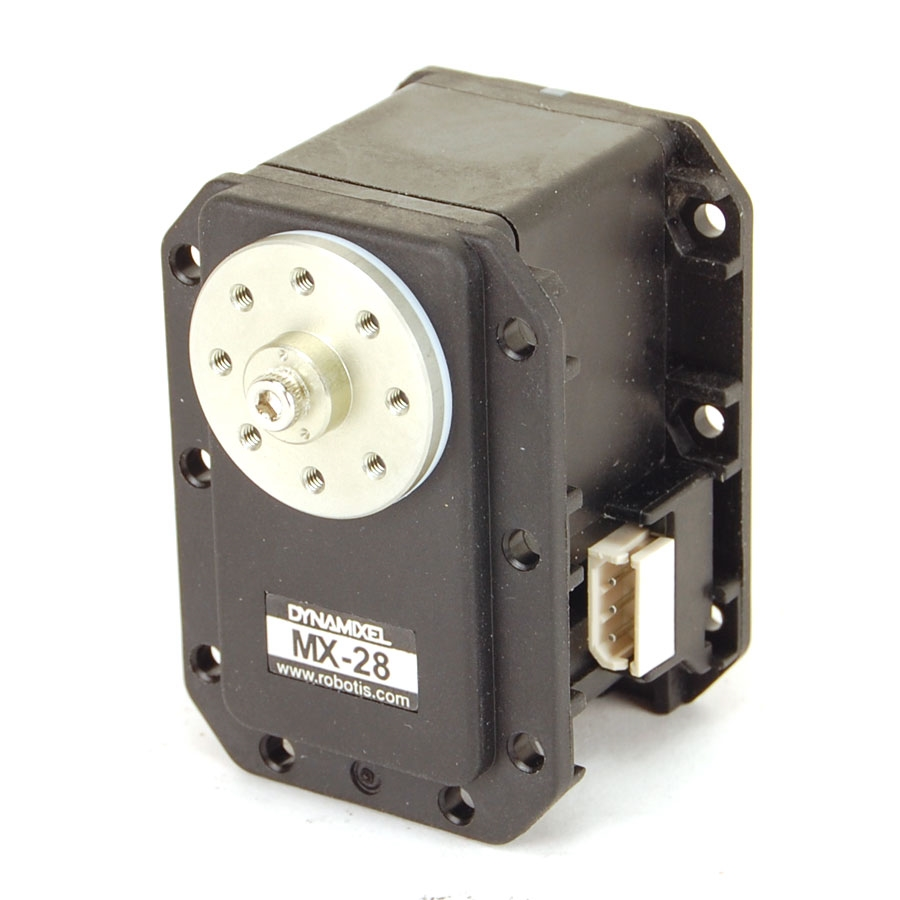
\includegraphics[width = \textwidth]{figures/mx28}
    \caption{MX-28R servo.}
    \label{fig:mx28_real}
\end{subfigure}
\hfill
\begin{subfigure}[b]{0.3\textwidth}
    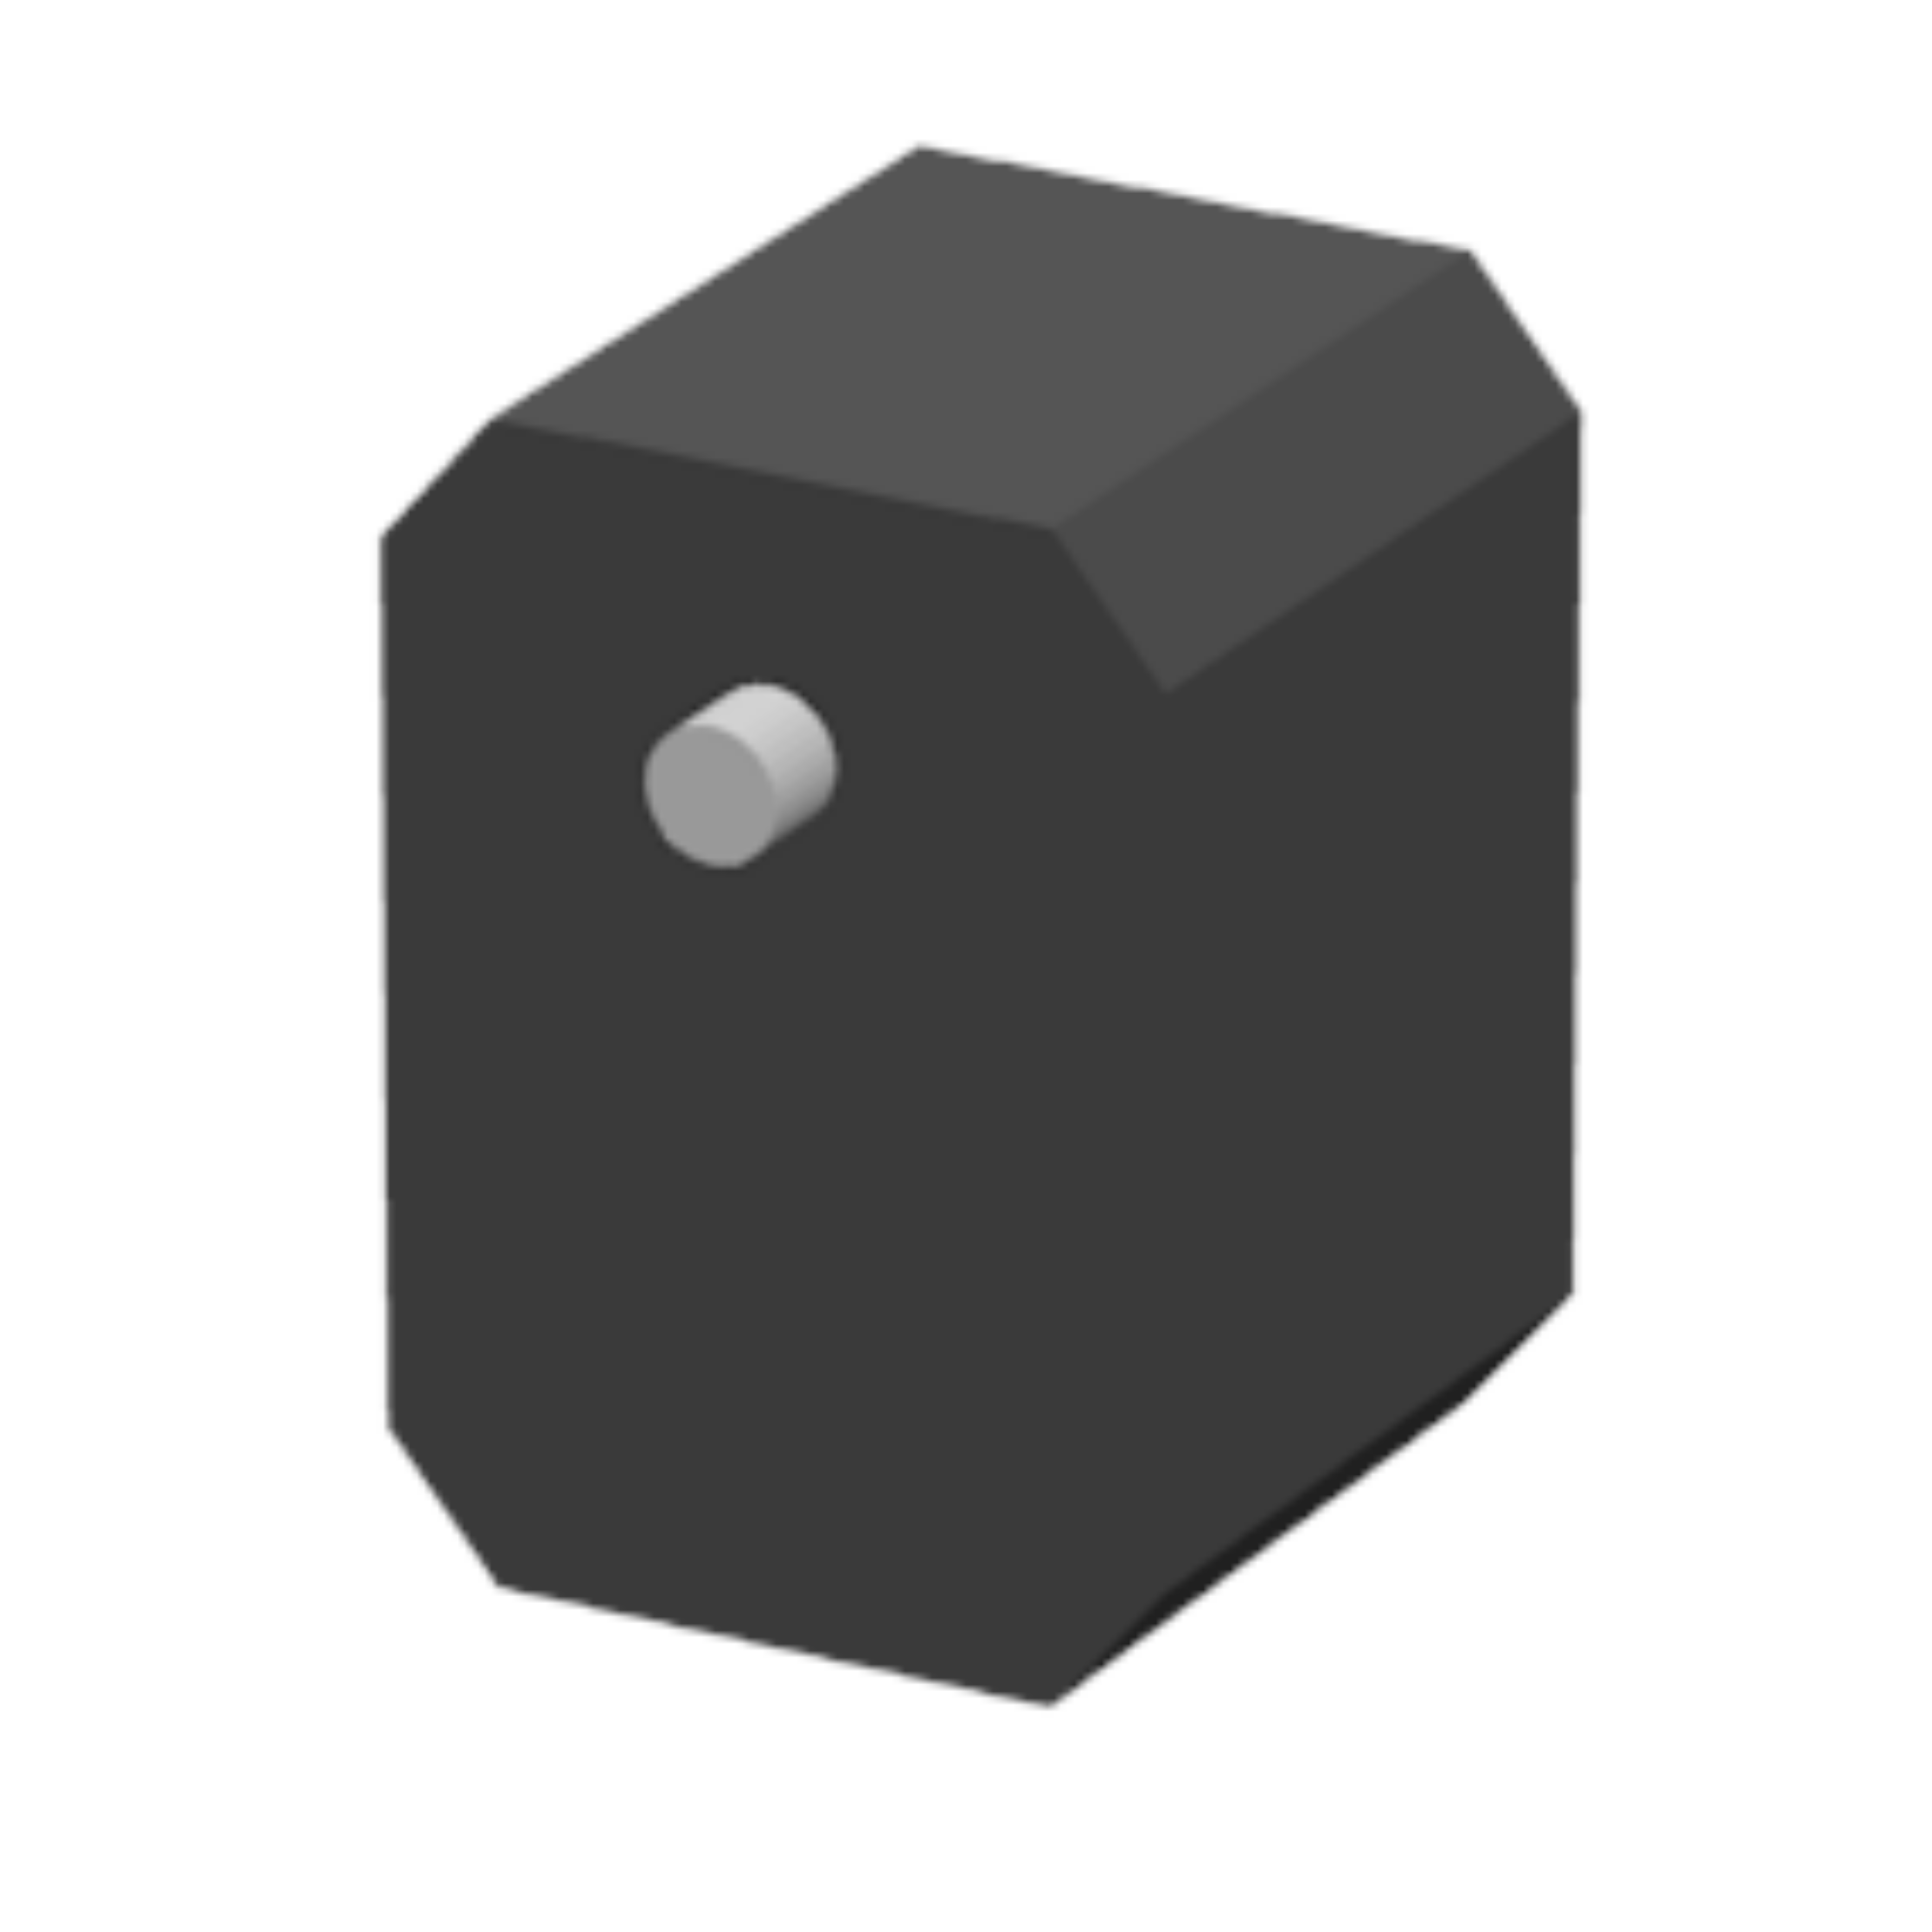
\includegraphics[width = \textwidth]{figures/mx28_model}
    \caption{Model of the MX-28R.}
    \label{fig:mx28_model}
\end{subfigure}
\caption[Side by side of a MX-28R servo and its 3D model]{Side by side of a MX-28R servo and its 3D model. The shape has been simplified but retains outer appearance of the servo. The axis is used as a position marker and will be removed once the joint is in place.}
\label{fig:servo}
\end{figure}

When the joint is in place, we edit its properties to set in torque/force mode and tick both the motor and control loop boxes of the joint dynamic properties window of \Cref{fig:joint}. The maximum torque is set to $1.2Nm$ and the maximum rotation speed to $(48.33 \cdot 360) / 60 = 290 \degree/s$. The MX-28R uses a PID controller to reach and hold the target positions so we do not need to write a custom control script and can content ourselves with modifying the proportional and integral parameters. 

\begin{figure}[htp]
\centering
    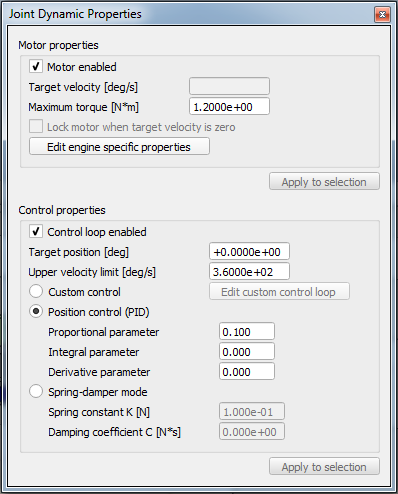
\includegraphics[width = 0.6\textwidth]{figures/joint}
    \caption[Dynamic properties of a revolute joint]{Dynamic properties of a revolute joint. When motor enabled we can set a target velocity along with a maximum torque and the joint acts as traditional motor. When the control loop is enabled the join acts as a servomotor and we can decide whether we use a PID controller or a custom control script.}
    \label{fig:joint}
\end{figure}

A PID controller is a feedback based control loop that is quite common in the engineering industry. An example of such a controller is the one that is implemented in the control code of the MX-28R that can be seen in \Cref{fig:mx28_pid}. The current position is measured and compared to the target position. The difference between those two is called the \emph{error}. The error then follows three parallel paths. In the first one it is multiplied by a \emph{proportional gain $K_p$}, which accounts for the present error. In the second one, it is integrated and multiplied by an \emph{integral gain $K_i$} which accounts for the past errors. It is used to counter steady-state errors that are not countered by the proportional error. It will accumulate and the integral error will eventually be high enough to counter that offset. The last one is derived and multiplied by a \emph{derivative gain $K_d$}. This gain accounts for the possible future values of the error and influences how fast the controller reacts. For more information on PID controllers and their use we please refer to \cite{johnson2005pid}.

\begin{figure}[htp]
\centering
    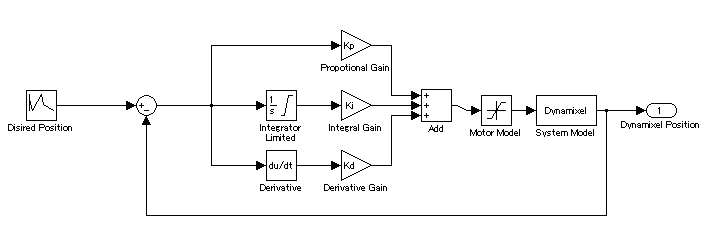
\includegraphics[width = \textwidth]{figures/pidcontrol}
    \caption[MX-28 PID controller]{Block diagram of the PID controller implemented in the MX-28R. It is a standard PID controller although by default only the P parameter is non-zero. The function of the \textit{motor model} block is to clamp the computed correction torque in the allowed interval whereas the \emph{system model} block is a simulink representation of the MX-28R and does not exist in the actual implementation inside the latter. Source: \cite{mx_28_manual}}
    \label{fig:mx28_pid}
\end{figure}

\clearpage
\section{Robot model}
The elements we just modelled can be assembled together to create the robot model in \Cref{fig:robotv7}. The next chapter will focus on simulations involving this model.
 
\begin{figure}[htp]
\centering
\begin{subfigure}[b]{0.64\textwidth}
    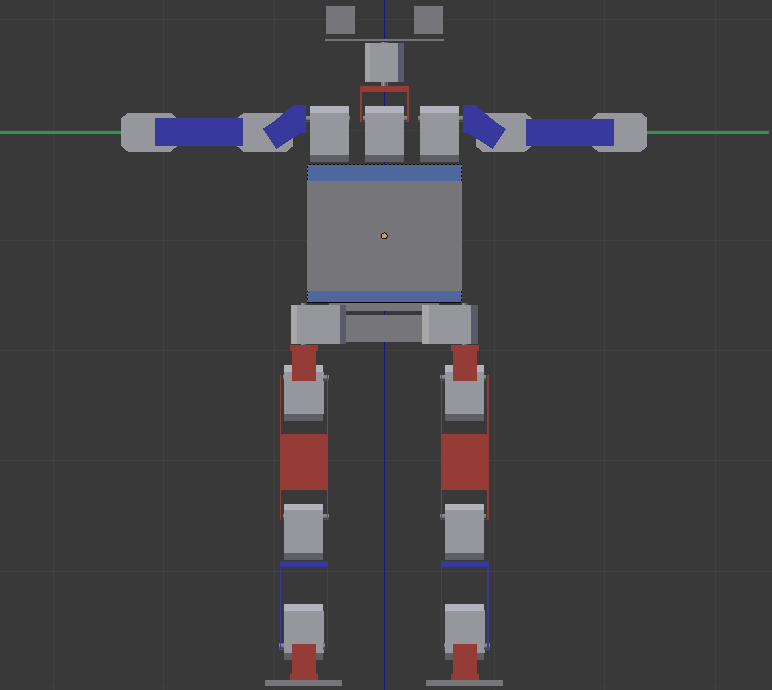
\includegraphics[width = \textwidth]{figures/robot_v7_front}
    \caption[]{Front view of the robot.}
    \label{fig:robotv7_front}
\end{subfigure}

\begin{subfigure}[b]{0.64\textwidth}
\centering
    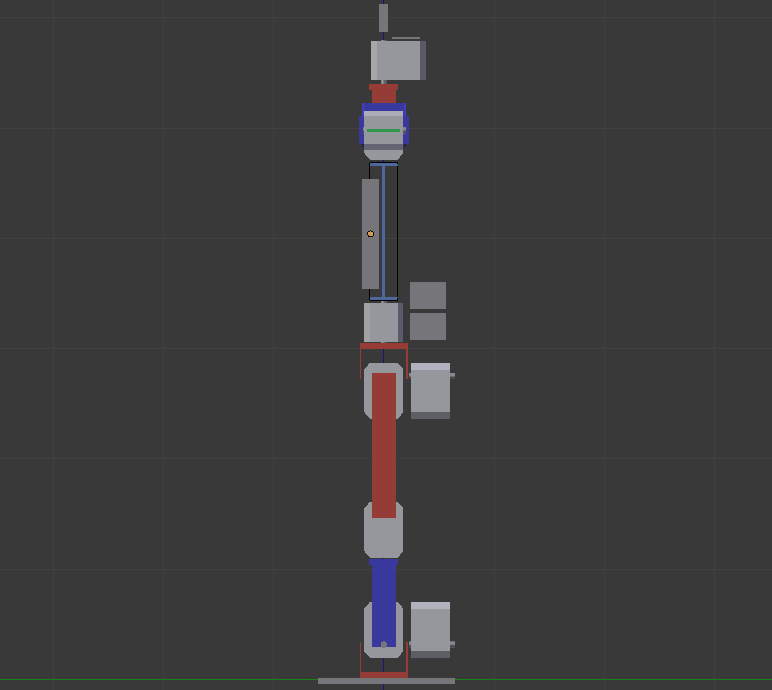
\includegraphics[width = \textwidth]{figures/robot_v7_side}
    \caption[]{Side view of the robot.}
    \label{fig:robotv7_side}
\end{subfigure}
\caption[Final robot model]{Front and side views of the final robot model to be used in the simulations in \cref{chap:simulation}.}
\label{fig:robotv7}
\end{figure}